\chapter{Use Cases}

\section{Introduction}
This section describes the four to five main use cases that a student can perform. The first subsection contains a diagram displaying the main user and the user's four to five possible actions. The second subsection details the name, goal, conditions, and steps corresponding to each use case. 

\section{Diagrams}
\begin{figure}[!ht]
      \centering
      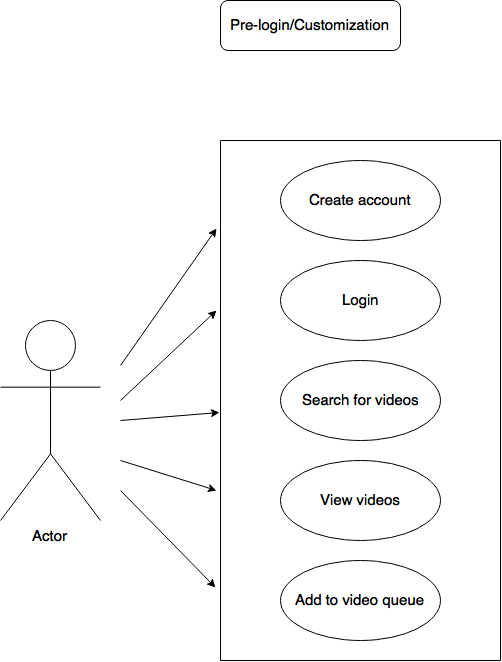
\includegraphics[width=0.5\textwidth]{useCasePreLogin}
      \caption{Use Case Diagram of Pre-login}	
\end{figure}
\begin{figure}[!ht]
      \centering
      \includegraphics[width=0.5\textwidth]{useCasePostLogin}
      \caption{Use Case Diagram of Post-login}	
\end{figure}


\section{Use Case Description}
\begin{itemize}
\item Create account
	\begin{itemize}
	\item Name: Create an account to be used on website
    \item Goal: To create an account ti be used on website
    \item Actor: User
    \item Preconditions
		\begin{enumerate}
		\item User must be on webpage
        \end{enumerate}
    \item Steps
    	\begin{enumerate}
		\item User selects my settings
        \item User selects create an account 
        \item User enters desired username and password combination
        \item User submits username and login combination to system to be submitted
        \end{enumerate}
    \item Post-conditions
		\begin{enumerate}
		\item Assuming user's username is unique, the combination gets committed to the system
        \item The website loads user's stored data and allows for user customization 
        \item The website returns to the overall view of the website with user now logged-in
        \end{enumerate}
    \item Exceptions
    	\begin{enumerate} 
    	\item User's username needs to be unique so process may need to be repeated to achieve a unique result, user will be alerted of error occurring 
        \end{enumerate}
    \end{itemize}

\item Login
	\begin{itemize}
	\item Name: Login to website
    \item Goal: To sign in to website
    \item Actor: User
    \item Preconditions
		\begin{enumerate}
		\item User must be on webpage
        \item User must have a preexisting account
        \end{enumerate}
    \item Steps
    	\begin{enumerate}
		\item User selects my settings
        \item User can create an account to be used to login
        \item User enters login credentials
        \item User submits login to be signed into website
        \end{enumerate}
    \item Post-conditions
		\begin{enumerate}
		\item User's username is checked if it exists in the system
        \item The matching username and password are returned 
        \item The user's password is then checked against the returned username's password
        \item Assuming the credentials match, the user is then logged on to the system
        \end{enumerate}
    \item Exceptions
    	\begin{enumerate} 
    	\item User who has entered information but has not created an account will be asked to create an account
        \end{enumerate}
    \end{itemize}
    
\item Search for Videos
	\begin{itemize}
	\item Name: Search for videos 
    \item Goal: Allows user to specify videos to watch
    \item Actor: User
    \item Preconditions
		\begin{enumerate}
		\item User must be entered into system
        \end{enumerate}
    \item Steps
    	\begin{enumerate}
		\item User types into textbox to specify which sports video to view
        \item User video returned ready to view
        \end{enumerate}
    \item Post-conditions
    	\begin{enumerate}
		\item User continues on website to view video
        \end{enumerate}
    \item Exceptions
    	\begin{enumerate}
    	\item Video requested by the user is unavailable in database of video sources, so user is alerted of unavailability of video and can re-enter search items to perform another search
    	\end{enumerate}
    \end{itemize}

\item View Videos
	\begin{itemize}
	\item Name: View videos 
    \item Goal: To watch video on website
    \item Actor: User
    \item Preconditions
		\begin{enumerate}
		\item User must be entered into system
        \item User must allow video to play
        \end{enumerate}
    \item Steps
    	\begin{enumerate}
		\item User able to enjoy video playback
        \end{enumerate}
    \item Post-conditions N/a
    \item Exceptions N/A
    \end{itemize}
    
\item Add to Video Queue
	\begin{itemize}
	\item Name: Add videos to queue
    \item Goal: To use website to add user specific videos to queue
    \item Actor: User
    \item Preconditions
		\begin{enumerate}
		\item User must be entered into system
        \item User must have already searched for videos
        \end{enumerate}
    \item Steps
    	\begin{enumerate}
		\item User types into textbox to specify which sports video to view
        \item Video is added to the back of the queue
        \item Video is ready to be viewed in queue order
        \end{enumerate}
    \item Post-conditions
    	\begin{enumerate}
		\item To view video user must allow video to play through
        \end{enumerate}
    \item Exceptions
    	\begin{enumerate}
    	\item If the user has cleared their queue of videos after the new video is added to the queue then the recently added video along with other videos queued for viewing will be removed from queue. System will play the newest video added next
    	\end{enumerate}
    \end{itemize}
    
\item Customize Settings
	\begin{itemize}
	\item Name: Customize settings
    \item Goal: To customize personal settings
    \item Actor: User
    \item Preconditions
		\begin{enumerate}
		\item User must be entered into system
        \item User must have an account and be logged into system
        \end{enumerate}
    \item Steps
    	\begin{enumerate}
		\item User clicks my settings tab
        \item User can edit their username and password
        \end{enumerate}
    \item Post-conditions
    	\begin{enumerate}
		\item User must save changes made when editing their profile
        \end{enumerate}
    \item Exceptions
    	\item *unable to udpate*
    \end{itemize}
    
\item View Customized Videos
	\begin{itemize}
	\item Name: View customized videos 
    \item Goal: To view list of customized videos referred to as MyReplay
    \item Actor: User
    \item Preconditions
		\begin{enumerate}
		\item User must be entered into system
        \item User must be logged into system
       	\item User must have edited and saved their MyReplay preferences
        \end{enumerate}
    \item Steps
    	\begin{enumerate}
		\item User returns back to home page of website
        \item User can enjoy video playback of queue
        \end{enumerate}
    \item Post-conditions
    	\begin{enumerate}
		\item The program grabs the desired data entries
        \item Videos will play in most recent found from database
        \end{enumerate}
    \item Exceptions
    	\begin{enumerate}
    	\item User may watch an old video if the update has not been run by program
    	\end{enumerate}
    \end{itemize}
    
\item Sign Out
	\begin{itemize}
	\item Name: Sign out of website
    \item Goal: To sign out the users profile from the website
    \item Actor: User
    \item Preconditions
		\begin{enumerate}
		\item User must be entered into system
        \item User must be signed in to the system
        \end{enumerate}
    \item Steps
    	\begin{enumerate}
		\item User clicks my settings tab
        \item User clicks log off button
        \item User profile has exited the system
        \end{enumerate}
    \item Post-conditions
    	\begin{enumerate}
		\item Clear user data from the website
        \item Reset the website so it functions as if a new user has just entered 
        \end{enumerate}
    \item Exceptions N/A
    \end{itemize}
    
\end{itemize}